%%%%%%%%%%%%%%%%%%%%%%%%%%%%%%%%%%%%%%%%%%%%%%%%%%%%%%%%%%%%%%%%%%
%%%%%%%% ICML 2014 EXAMPLE LATEX SUBMISSION FILE %%%%%%%%%%%%%%%%%
%%%%%%%%%%%%%%%%%%%%%%%%%%%%%%%%%%%%%%%%%%%%%%%%%%%%%%%%%%%%%%%%%%
\documentclass{article}
\usepackage{times}
\usepackage{graphicx} % more modern
\usepackage{subfigure} 
% For citations
\usepackage{natbib}
% For algorithms
\usepackage{algorithm}
\usepackage{algorithmic}

% Stuff that I added in (Daniel Seita) 
\usepackage{amsmath,amssymb,amsthm,enumitem,verbatim}
\graphicspath{ {Images/} }
\newtheorem{thm}{Theorem}[section]
\newtheorem{conj}[thm]{Conjecture}
\newtheorem{cor}[thm]{Corollary}
\newtheorem{lem}[thm]{Lemma}
\newtheorem{prop}[thm]{Proposition}
\newtheorem{exa}[thm]{Example}
\newtheorem{defi}[thm]{Definition}
\newtheorem{exe}[thm]{Exercise}
\newtheorem{rek}[thm]{Remark}
\newtheorem{que}[thm]{Question}
\newtheorem{prob}[thm]{Problem}
\newtheorem{cla}[thm]{Claim}
% End of stuff I added in

% As of 2011, we use the hyperref package to produce hyperlinks in the resulting PDF.  If this breaks your system, please commend out the following
% usepackage line and replace \usepackage{icml2014} with \usepackage[nohyperref]{icml2014} above.
\usepackage{hyperref}

% Packages hyperref and algorithmic misbehave sometimes.  We can fix this with the following command.
\newcommand{\theHalgorithm}{\arabic{algorithm}}

% Employ the following version of the ``usepackage'' statement for submitting the draft version of the paper for review.  This will set the note in
% the first column to ``Under review.  Do not distribute.''
%\usepackage{icml2014} 
% Employ this version of the ``usepackage'' statement after the paper has been accepted, when creating the final version.  This will set the note in
% the first column to ``Proceedings of the...''
\usepackage[accepted]{icml2014}

% The \icmltitle you define below is probably too long as a header.  Therefore, a short form for the running title is supplied here:
\icmltitlerunning{The Distributed Retired Traveling Salesman Problem}

\begin{document} 

\twocolumn[
\icmltitle{The Distributed Retired Traveling Salesman Problem}

% It is OKAY to include author information, even for blind submissions: the style file will automatically remove it for you unless you've provided the
% [accepted] option to the icml2014 package.
\icmlauthor{Daniel Seita}{dts1@williams.edu}
\icmlauthor{Ziang Zhang}{zz2@williams.edu}
\icmladdress{Department of Computer Science, Williams College, Williamstown, MA 01267 USA}

% You may provide any keywords that you find helpful for describing your paper; these are used to populate the "keywords" metadata in the PDF but will
% not be shown in the document
\icmlkeywords{distributed systems}

\vskip 0.3in
]

\begin{abstract} 
The use of major online travel agencies has made scheduling long-term travel much easier by allowing users to easily identify a set of flights in just
a few clicks. Current travel agencies allow users to plan out long-term trips involving flights to more than two cities, but they require specific
arrival and departure dates for each city and a city ordering. We present a system that does not burden the user with these decisions. Specifically,
our code takes in two required inputs: a list of cities the user wishes to travel to, and a date range over which they are willing to travel, and
outputs the cheapest set of flights within that range that form a valid route. It essentially solves a harder version of the Traveling Salesman
Problem since costs are not constant between two cities. Under several weak assumptions, and assuming that the number of cities and days is
sufficiently limited, then our algorithm should successfully find the cheapest cost flight in a reasonable amount of time. We present the theoretical
and systematic components of the project and discuss empirical results.
\end{abstract} 

\section{Introduction and Motivation}\label{sec:intro}

The use of major online travel agencies, such as Travelocity\footnote{\url{www.travelocity.com}} and Kayak\footnote{\url{www.kayak.com}}, has made
scheduling long-term travel much easier by allowing users to easily select a set of flights to purchase tickets from. People use a combination of
factors to help them make their decision, such as the total price of the flights and the days they wish to land and depart from a city. Current travel
agencies allow users to plan out trips involving airlines to multiple destinations (see Figure~\ref{fig:travelocity} for an example using
Travelocity), but they require (1) specific dates for each city and (2) an ordering.

This limitation can make searching for flight routes time-consuming for users who are not restricted to arriving at cities on particular dates. For
instance, suppose one resides in New York City (NYC) and wants to schedule a summer trip to Paris, London, and Tokyo from June 1 to June 20, and it
does not matter to him how long he stays in a city. Suppose that it also does not matter the ordering that he arrives at the cities. Thus (for now) we
will only care about the following factors\footnote{For brevity, we list a high-level overview of the problem without getting into too many technical
details; Section~\ref{sec:limitations} describes some of our assumptions and limitations.}:

\begin{itemize}[noitemsep]
    \item The full flight route occurs within the date range (in this case, between June 1 and June 20).
    \item The flight route must arrive and leave at least once for NYC, Paris, London, and Tokyo.
    \item The flight route is valid and logically consistent. For instance, if the first flight takes him from NYC to Tokyo, the second flight in the
    route should not depart from a place other than Tokyo.
\end{itemize}

There are a vast pool of valid flight routes. We might assume that out of all these, one would want the \emph{cheapest} route. Of course, this glosses
over how the user may want to spend some number of days at each city, but this is the most general case.

Unfortunately, finding the cheapest route possible is challenging using current agencies, because they require knowing the arrival and departure dates
for each city. The reason for this is simple: the problem of finding this flight route is a hard problem to solve. In fact, this problem is very
similar to the well-known Traveling Salesman Problem~\cite{Applegate:2007:TSP:1374811}, which asks if there exists a cycle in a graph that touches
each node exactly once (i.e., a Hamiltonian cycle). Each edge has a cost associated with it, and the decision version of the problem, which asks if
there exists a valid Hamiltonian cycle with cost bounded by $B$, is NP-complete~\cite{Kar72}. In our case, we do not force the user to visit each
city exactly once because the cheapest flight through a sequence of cities \emph{may require} visiting a city more than once.

What makes our problem (likely) much harder than the Traveling Salesman Problem is that the cost of an edge between two nodes in our graph (i.e., two
cities) is not constant, because flight prices frequently change. We coin our problem the ``Distributed Retired Traveling Salesman Problem.'' The
``Retired'' portion comes from how we assume that whoever is planning this trip is retired, because otherwise, how would he or she have the time and
money? The ``Distributed'' part is because we incorporate concepts from the design and practice of distributed systems to build software that can
tackle this problem. We discuss the mathematical and systems portions of our solution in Sections~\ref{sec:math} and~\ref{sec:systems}, respectively.

\begin{figure}[t]
\vskip 0.2in
\begin{center}
\centerline{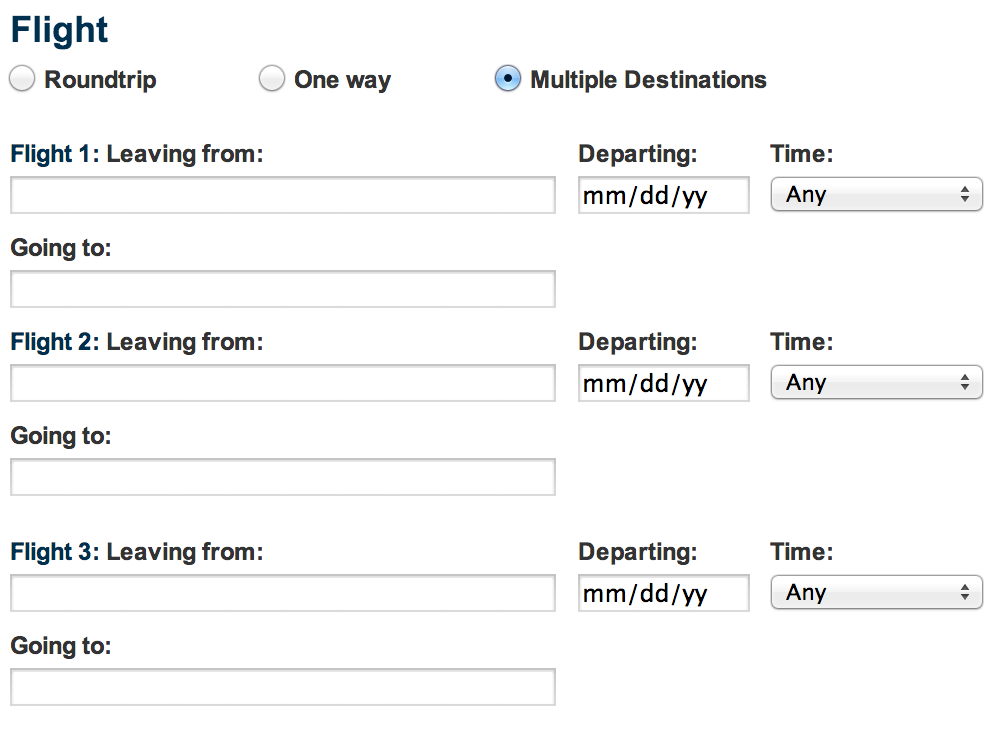
\includegraphics[width=\columnwidth]{travelocity}}
\caption{Travelocity lets users select multiple destinations.}
\label{fig:travelocity}
\end{center}
\vskip -0.2in
\end{figure}

\section{Related Work}\label{sec:related_work}

The Traveling Salesman Problem (TSP) is one of the oldest and most well-known problems in combinatorial optimization. While no exact, polynomial time
solution for the decision problem is known, there is a $3/2$-approximation algorithm due to Christofides~\cite{Chr76}. That algorithm was long the
standard approximation algorithm until a stunning recent result in~\cite{conf/focs/GharanSS11}, which has thus spurred a cascade of additional
research relating to the TSP (e.g.,~\cite{Moemke:2011:AGT:2082752.2082898}).

In contrast to the attention devoted to TSP, there appears to be very little research focusing on the special case of our problem, which introduces
additional challenges. These can be mathematically-oriented, such as how to manage the variable costs, or systems-oriented, such as how to even obtain
the actual flight costs. We have found nothing in the literature that particularly fits our problem.

\section{Mathematical Component}\label{sec:math}

The mathematical portion of our work uses a technique known as \emph{binary integer linear programming}, which falls under the broader category of
optimization techniques. The goal in optimization is straightforward: given a set of variables and a set of constraints, the goal is to find the best,
feasible solution according to some criteria, such as cost (in which case, ``best'' means ``minimal'').

\subsection{Linear and Integer Programming}\label{sec:lin_int_programming}

One of the most commonly-used optimization techniques is linear programming, introduced by Dantzig in~\cite{GVK180926950}.

\begin{defi}\label{defi:linear_programming}
A \emph{linear programming problem} consists of three components: 
\begin{enumerate}[noitemsep]
    \item a finite collection of linear inequalities or equations in a finite number of unknowns, $x_1, \ldots, x_n$;
    \item sign constraints $x_i \ge 0$ on some (possibly empty) subset of the unknowns;
    \item a linear function to be minimized or maximized.
\end{enumerate}
An assignment to the variables $x_1, \ldots, x_n$ satisfying the first two conditions is a \emph{feasible} solution. If it also satisfies the third,
then it is an \emph{optimal} solution~\cite{opac-b1105716}.
\end{defi}

Linear programming has tremendous applications, and a full list of them would be impossible to create. Some problems well-suited to linear programming
include investment management, scheduling problems, and the diet problem. (The last problem concerns the rather interesting question of what is the
minimum cost of a nutritionally adequate diet.) The reason for linear programming's great versatility is the ease at which constraints can be added to
a model.

More specific cases of linear programming are integer and binary linear programming. (Sometimes we drop the ``linear'' part for brevity.)

\begin{defi}\label{defi:integer_programming}
An \emph{integer programming problem} is a linear programming problem with the added restriction that all variables (i.e., unknowns) $x_1, \ldots,
x_n$ are integers.
\end{defi}

\begin{defi}\label{defi:binary_programming}
A \emph{binary integer programming problem} is an integer programming problem with the added restriction that all variables $x_1, \ldots,
x_n$ are such that $x_i \in \{0,1\}$.
\end{defi}

We see that our problem is particularly suited to binary integer programming, because all the possible flights we could take can be viewed as a set of
binary random variables, each of which has value 1 if we decide to take that flight, and 0 otherwise. We now formulate this problem in more detail.

\subsection{An Integer Programming Formulation}\label{sec:int_prog_form}

To start formulating the problem, we make it concrete what we mean by cities, days, and costs.

\begin{itemize}[noitemsep]
    \item We have $n$ cities to reach; we index cities by $i$ or $j$, where $i, j \in \{1, 2, \ldots, n\}$.
    \item We have $t$ consecutive days when we can travel: $t \in \{1, 2, \ldots, m\}$.
    \item The minimum cost for traveling from city $i$ to $j$ on day $t$ is $c_{ijt}$.
\end{itemize}

Using the above lets us define the following variables:

\[
x_{ijt} = \begin{cases}
1 &\mbox{if we go from cities } i \mbox{ to } j \mbox{ on day } t, \\ 
0 & \mbox{otherwise}.
\end{cases}
\]

Thus, a solution to our problem will be the full assignment to each of the above variables. The set of the binary variables that equal one will
(assuming the set has cardinality $k$) correspond to $k$ flights $f_1, \ldots, f_k$ ordered by date.

For now, we make several simplifying assumptions, and defer a more detailed discussion about the realism of this project in
Section~\ref{sec:limitations}. Perhaps the most important one is that we assume each flight is assigned to exactly one day. We will also force a valid
solution to have flights all on different days. This means, at the moment, we do not consider issues related to (1) overnight flights (we will pretend
they do not exist), (2) multiple-stop flights on the same day, and (3) possible logistic impossibilities such as flight $f_i$ arriving at 11:59 PM and
then the next flight $f_{i+1}$ departing from the same airport two minutes later (but on the next day).

The goal is to solve this minimization problem:

\begin{equation}
\mbox{Minimize } \sum_{t=1}^{m} \sum_{i=1}^{n} \sum_{j=1}^{n} c_{ijt}x_{ijt},
\end{equation}

\emph{subject to} the following constraints:
\begin{align}
\sum_{i=1}^{n} \sum_{j=1}^{n} x_{ijt} &\le 1 \mbox{ for all } t \in \{1, 2, \ldots, m\}, \\ 
\sum_{t=1}^{m} \sum_{i=1}^{n} x_{ijt} &\ge 1 \mbox{ for all } j \in \{1, 2, \ldots, n\}, \\
\sum_{t=1}^{m} \sum_{j=1}^{n} x_{ijt} &\ge 1 \mbox{ for all } i \in \{1, 2, \ldots, n\}.
\end{align}

The first constraint ensures that we have at most one flight per day, which is generally too restrictive for real-life, but will suffice for now. The
second constraint ensures we enter each city at least once. The third constraint ensures we leave each city at least once. These last two reinforce
the notion that going through the cheapest route may mean visiting several cities more than once.

Sadly, these previous constraints are \emph{not} enough to solve our problem. There are two glaring issues with the current constraints that, if we
were to use them to solve this flight scheduling problem, could result in a logically inconsistent flight route.

\subsubsection{Disjoint Cycles}\label{sec:disjoint_cycles}

The first problem is that the constraints do not prevent disjoint cycles. Figure~\ref{fig:bad_solution} shows a graph with six nodes, which may
represent six cities, and a possible edge assignment that is indicative of the route we take to visit all cities. Assuming the flights are all on
different days, the route satisfies our constraints, because we enter and exit each city at least once, but this is not a Hamiltonian cycle.

\begin{figure}[t]
\vskip 0.2in
\begin{center}
\centerline{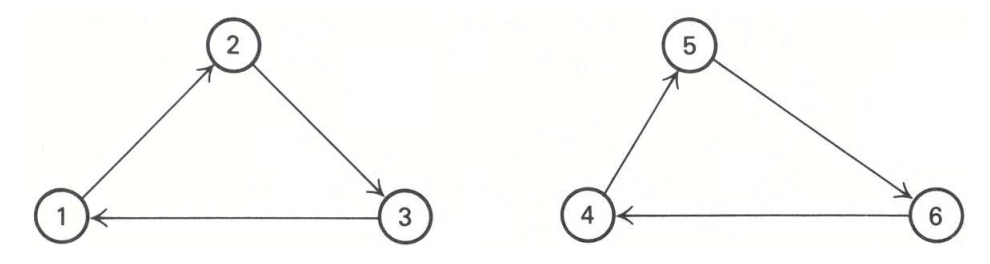
\includegraphics[width=\columnwidth]{bad_solution}}
\caption{This represents two sets of disjoint cycles.}
\label{fig:bad_solution}
\end{center}
\vskip -0.2in
\end{figure}

To prevent disjoint cycles, we need to add additional constraints that correspond to all the ways we can subdivide the cities into two groups so that
both of them contain at least two cities. (A subdivision where one group only has one city is already covered by our earlier constraints since we
would have to leave and enter that city at least once, which requires connecting with the other group.) For instance, with the six-variable situation
in Figure~\ref{fig:bad_solution}, one constraint would be
\begin{align}
\sum_{t=1}^{m} (&x_{14t} + x_{15t} + x_{16t} + x_{24t} + x_{25t} + \\
& x_{26t} + x_{34t} + x_{35t} + x_{36t}) \ge 1, \nonumber
\end{align}

which ensures that at least one leg of the tour connects cities 1, 2, and 3 with cities 4, 5, and 6, so this corresponds to the subdivision of
$\{[1,2,3],[4,5,6]\}$. We can characterize the number of constraints we need to add to prevent disjoint cycles.

\begin{lem}\label{lem:cycle_constraints}
In a problem that has $n \ge 4$ constraints, the number of ways to subdivide the cities so that each has two groups is ${n \choose 2} + {n \choose 3}
+ \cdots + {n \choose n-2}$.
\end{lem}

The reasoning is straightforward: we have two groups, and we want to pick the number of elements for one group. We can pick some number out of $n$
elements to be in one group, and assign all the rest to the others.

One technical note is that the number of constraints from Lemma~\ref{lem:cycle_constraints} can be halved by symmetry. Still, the number of equations
needed grows rapidly with respect to $n$, and the need to implement these various restrictions is why integer programming is a hard task. Integer
programming is, in fact, an NP-hard problem, and the binary case is NP-complete~\cite{Kar72}. In contrast, faster algorithms such as the Simplex
method\footnote{The Simplex Method performs well in practice but its runtime has historically been difficult to evaluate, as in the worst case it
\emph{can} run in exponential time~\cite{Klee1972}. The simplex algorithm has \emph{smoothed complexity} polynomial in the input size; for details
about this, see~\cite{Spielman:2004:SAA:990308.990310}.} are used to solve linear programming problems. Note that simply taking a solution to the
linear programming problem and then rounding it to form a ``solution'' to the integer problem will not work, as we show in Section~\ref{app:lin_vs_int}.

\subsubsection{Consecutive Flights in Different Cities}

The second problem with the constraints posed earlier in Section~\ref{sec:int_prog_form}, which the constraints in~\ref{sec:disjoint_cycles} do
\emph{not} resolve, is that we can get flight orderings that are logically inconsistent in the sense that consecutive flights may not agree in their
choice of cities. It makes no sense, for instance, to have flights $f_i$ and $f_{i+1}$ where $f_i$ takes the participant from NYC to Tokyo, and
$f_{i+1}$ takes him or her from Paris to London.

Unfortunately, fixing the flight ordering by adding in constraints is challenging and requires a large number of equations. Our implementation only
adds in one layer of constraints for here, and defers a complete flight logic check to the code that actually generates the tree. Thus, we resolve
this by just solving the problem as we would normally without the constraint, and then checking all proposed solutions for flight logic before
accepting them.

For more details about this, see Section~\ref{app:flight_logic}.

{\bf TODO}

\subsection{Using Balas' Additive Algorithm}\label{sec:balas}

We will use this algorithm to solve Integer Programming. See~\cite{doi:10.1287/opre.13.4.517}.

{\bf TODO}




\section{Systems Component}\label{sec:systems}

Our code that solves the Distributed Retired Traveling Salesman Problem is made up of several components that form a multi-tiered client-server model
(for an introduction to the client-server model, see~\cite{Tanenbaum:2006:DSP:1202502}).  We have a front-end server, a master server, and a group of
slave servers in the system, as shown in Figure~\ref{fig:machines}. The slave servers come from machines that we use. Originally, we wanted to use
PlanetLab~\cite{conf/osdi/PetersonBFM06}, which is a global platform for deploying and evaluating network services and allows people to use portions
of other PlanetLab computers. This was too complicated to work with, so we stuck with the Williams lab computers.

{\bf TODO}

\begin{figure}[t]
\vskip 0.2in
\begin{center}
\centerline{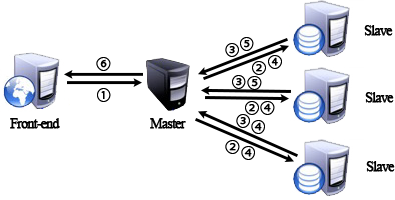
\includegraphics[width=\columnwidth]{servers}}
\caption{This represents our setup.}
\label{fig:machines}
\end{center}
\vskip -0.2in
\end{figure}

\subsection{Front-end Server}\label{sec:front_end_server}

The front-end server acts as a point of communication between the client\footnote{Somewhat impolitely, we can refer to the set of clients, minus us,
as the ``ignorant masses.''} and our master server. It is a Python script that starts on the command line and outputs introductory messages to the
client so that he or she knows how to use our system. The front-end serve receives user input, forwards the request to the master server (step
\texttt{1} in Figure~\ref{fig:machines}), listens to the master for the result (step \texttt{6} in Figure~\ref{fig:machines}), and displays the result
when it is ready. The result that we print back to the user is currently the single best list of the flights ordered by departure date. If there is
more than one optimal solution, it only returns one of them.

\begin{figure}[t]
\vskip 0.2in
\begin{center}
\centerline{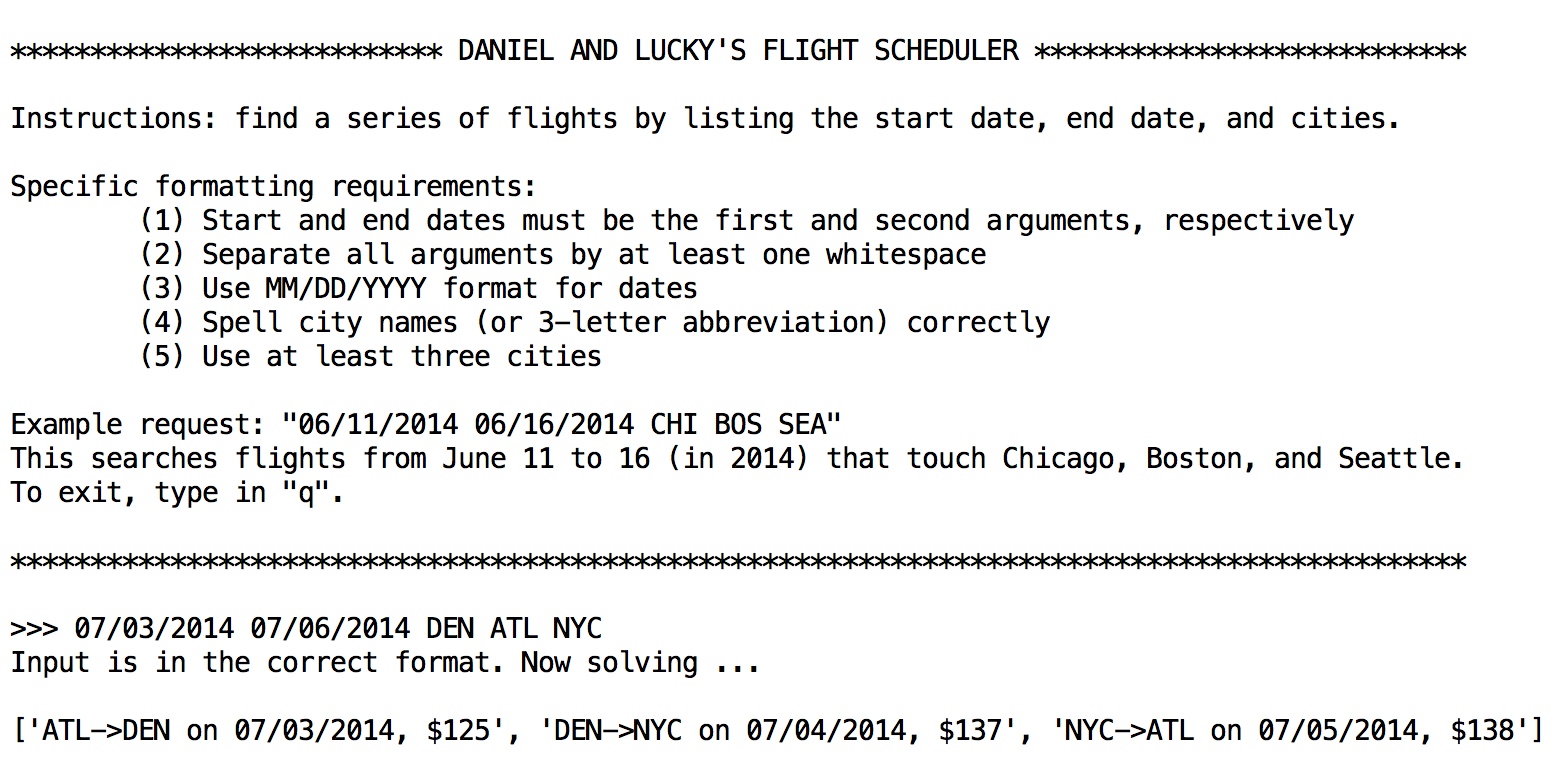
\includegraphics[width=\columnwidth]{front_end_server}}
\caption{This shows our front-end server.}
\label{fig:front_end_server}
\end{center}
\vskip -0.2in
\end{figure}

Figure~\ref{fig:front_end_server} shows a version of our front-end server (we change its design fairly frequently). Here, the hypothetical user made a
request to find the cheapest flight route that touches Denver, Atlanta, and New York City from the four day period of July 3, 2014 to  July 7, 2014.
Our code ran and the master server fed back the resulting flight ordering of Atlanta to Denver, then Denver to New York City, then New York City back
to Atlanta.

If time permits, we may transform the command-line interface to a website, which will expand our audience of potential clients. It is also
straightforward to add more optional arguments to the command line, so the user might add in an extra flag that could indicate that he or she wishes
to have a minimum of three days between flights.


\subsection{Master Server}\label{sec:master_server}

The Master server is the brain of the system. It listens to the user request sent from the front-end server (step \texttt{1} in
Figure~\ref{fig:machines}). When a request comes in, it first comes up with a list of flight prices on all possible dates and for all possible
destinations in the problem that we need to get for the computation, distributes the flight price queries among all the slaves (step \texttt{2}),
gathers all the price data back from the slaves (step \texttt{3}), and combines them. It then upload the combined data to a distributed file system to
make the data available for parallel computing on all the slaves. Then it starts the parallel computing for the cheapest route using a distributed
zero-one linear programming algorithm on all slaves (steps \texttt{4} and \texttt{5}). After the computation, it sends the results of the cheapest
route back to the front-end server (step \texttt{6}).

{\bf TODO! This needs more information.}

\subsection{Slave Server}\label{sec:slave_server}

We have a group of slave servers that listens to the command of the master server and does the distributed tasks of flight price querying (using the
web crawler we write) and parallel zero-one linear programming.

The slave server uses this! Be clear on that!

We will use the Matrix Airfare Search\footnote{\url{http://matrix.itasoftware.com/}} database to obtain information about our flights; the information
itself will be extracted with our own web crawler. We coin this ``The Retired Traveler Problem,'' primarily because if we assume the dates are set far
enough apart, it would interfere with a non-retired person's occupation. For details on the real problem, see sources such as.

{\bf TODO! This needs more information.}


\section{Experiments and Results}\label{sec:experiments_results}

{\bf TODO}

\subsection{Simple Examples}
{\bf TODO}

\subsection{Runtime Analysis}
{\bf TODO}

\subsection{Feasibility}
{\bf TODO}


\section{Limtiations}\label{sec:limitations}

{\bf TODO}

\subsection{One Flight a Day}
{\bf TODO}

Explain that matrix ita will sometimes give us two or three flights for ``one route'' so it actually works out ok...in some ways.

\subsection{One Ticket, Multiple Flights}
{\bf TODO}

Explain that this will give us problems.

\section{Conclusion}\label{sec:conclusion}

We view this as a beginning, rather than an end, of the Distributed Retired Traveling Salesman Problem. There are several ways of proceeding from our
work.

\begin{itemize}\label{noitemsep}
    \item We could improve the aesthetics of our implementation. Most prominently, our front-end server is in the form of a command-line interface,
    but many people do not know how to use those. Consequently, we could reach out to and would be much more comfortable with a streamlined website.
\end{itemize}

Overall, this was an extremely fun project. It was one of the most successful projects where we had only a vague plan but ended up with hopefully a
working implementation that could be useful under the right circumstances.

{\bf TODO}

\section*{Acknowledgments}
 
We thank Brent Heeringa for introducing us to the world of NP-completeness, Jeannie Albrecht for teaching us how to play around with servers and
design distributed systems, and Steven Miller for carving out time from his super-busy schedule to provide us with an independent study that gave us
the requisite mathematical background.

\bibliography{Daniel_Lucky_Report}
\bibliographystyle{icml2014}








% Jeannie doesn't need to read this if she doesn't want to...
\onecolumn

\appendix

\begin{center}
{\Large \textbf{Supplementary Material}}
\end{center}

Outline of Supplementary Material:

\begin{itemize}[noitemsep]
    \item TODO
    \item TODO
    \item TODO
    \item TODO
\end{itemize}


\section{Integer Programming versus Linear Programming}\label{app:lin_vs_int}

Here, we should describe the interaction between integer and linear programming, and show why integer programming is harder and cannot be obtained by
rounding from the linear solution. Our work, of course, is heavily influenced by~\cite{stevenmiller}.

{\bf TODO}

\section{Adding Constraints to Prevent Flight Logic Errors}\label{app:flight_logic}

Here, we should describe the constraints that we added in for flight logic. I only added in one layer of constraints.

{\bf TODO}

\section{Balas' Additive Algorithm}\label{app:balas}

{\bf TODO}

\section{Additional Experiments and Examples}\label{app:additional_experiments_and_examples}

{\bf TODO}

% Daniel's stuff for experimentation. Do not include these in the final document.

\end{document} 




% Look at that! Andrea is here! ~Daniel Seita (05/08/2014)

% This document was modified from the file originally made available by
% Pat Langley and Andrea Danyluk for ICML-2K. This version was
% created by Lise Getoor and Tobias Scheffer, it was slightly modified  
% from the 2010 version by Thorsten Joachims & Johannes Fuernkranz, 
% slightly modified from the 2009 version by Kiri Wagstaff and 
% Sam Roweis's 2008 version, which is slightly modified from 
% Prasad Tadepalli's 2007 version which is a lightly 
% changed version of the previous year's version by Andrew Moore, 
% which was in turn edited from those of Kristian Kersting and 
% Codrina Lauth. Alex Smola contributed to the algorithmic style files.  
